\section{Experiments and Results}\label{sec:experiments_results}

In this section we will evaluate the proposed architecture for the head calibration system. We will perform simulated and real experiments to evaluate the system in terms of its accuracy and repeatability. The real experiments were performed using the iCub robotic platform, \cite{Metta08}, more specifically the head \cite{Beira06}. The iCub was developed in the context of the EU project RobotCub and was adopted by more than 20 laboratories worldwide. The full robot has 53 DOF with the head having 6 DOF from the neck to each of the eyes, as seen in figure \ref{fig:head_kinematic_model_prob_form}a).

For each joint the robot's head is equipped with relative encoders that are extremely precise but are unable to measure the absolute zero position of the joint. The head is also equipped with an Xsens IMU that measures the linear accelerations and angular velocities at a frequency of 100Hz. This sensor is placed on top of the head right before the eyes tilt joint, $\delta_3$, as seen in figure \ref{fig:head_kinematic_model_prob_form}a). Finally the head is equipped with two Pointgrey Dragonfly cameras, that work at 30Hz and provide RGB images with VGA resolution ($640\times480$pixel). These cameras have $4.7\times3.5$mm CCD sensors and a field of view of $87.3\degree$ (horizontal) and $70.8\degree$ (vertical). The cameras are the last sensors in the kinematic chain being affected by all the joints. The intrinsic parameters of the cameras were calibrated using the Bouguet Toolbox \cite{Bouguet08} and where the radial distortion was completely eliminated. The calibrated parameters are presented in table \ref{tab:intrinsic_parameters}.

\begin{table}
\centering
\begin{tabular}{ccc}
 \hline
 Parameter & Left Camera & Right Camera \\
 \hline
 Width (pixel) & $640$ & $640$\\
 Height (pixel) & $480$ & $480$ \\
 $f_x$ (pixel) & $332.706$ & $342.367$\\
 $f_y$ (pixel) & $382.658$ & $389.545$\\
 $c_x$ (pixel) & $348.316$ & $350.601$\\
 $c_y$ (pixel) & $241.872$ & $251.704$\\
 \hline\\
\end{tabular}
\caption{Intrinsic parameters of the cameras: resolution (Width and Height), focal lengths ($f_x$ and $f_y$) and optical centers ($c_x$ and $c_y$)}
\label{tab:intrinsic_parameters}
\end{table}

In order to validate the proposed architecture we performed simulated experiments where all the sensors measurements were simulated and fed to the system just like in the real case. For both cases, the simulated and real, we created multiple datasets. Each dataset contains information from all the sensors at every time step: the linear accelerations and angular velocities from the IMU, the motor encoders and stereo images from both cameras (or simulated image features in the simulation case).

The calibration procedure for the real case goes as follows: the motors are initialized at an arbitrary position and we start the data acquisition while randomly rotating the head, as seen in figure \ref{fig:head_calibration_procedure}. Several datasets were acquired either for the same encoders offsets and for different encoders offsets, to completely evaluate the system in terms of its accuracy and repeatability.

\begin{figure}
    \centering
    \begin{tabular}{ccc}
        \includegraphics[width=0.275\columnwidth]{images/pos_1} &  
        \includegraphics[width=0.275\columnwidth]{images/pos_2} & 
        \includegraphics[width=0.275\columnwidth]{images/pos_3} \\
        \includegraphics[width=0.275\columnwidth]{images/pos_4} &  
        \includegraphics[width=0.275\columnwidth]{images/pos_5} & 
        \includegraphics[width=0.275\columnwidth]{images/pos_6} \\
    \end{tabular}
    \caption{The head calibration procedure where the head is initialized at a random position and is rotated in order acquire data for the different experiments.}
    \label{fig:head_calibration_procedure}
\end{figure}

To initialize the system state uncertainty as well as the transition process noise we took into consideration the nature of the problem. We are estimating joint offsets that must be combined with the encoders values to provide calibrated measurements. We are initializing the system state with the first observations received from the encoders, as soon as the calibration system starts to run. For this reason, we have a large uncertainty at the beginning considering the physical limits of each joint. To ensure the system's convergence, the state's initial uncertainty must be large enough to include all the possible values the offsets could take. Therefore we initialized each offset uncertainty with a large value, $40$deg. The transition process noise was set to $0.05$deg, so it could adapt to sudden changes while keeping the estimates as constant as possible.

We analysed the noise levels that described each of the sensors' measurements, assumed to be zero mean Gaussian noise. The standard deviations values are represented in table \ref{tab:sensors_noise}.

\begin{table}
\centering
\begin{tabular}{ccc}
 \hline
 Sensor Measurement & Noise Std. Dev & Frequency (Hz) \\
 \hline
 Linear Acceleration & $0.0447m/s^2$ & $100$\\
  Angular Velocities & $0.5$deg/s & $100$\\
  Encoders & $0.028$deg & $>100$\\
  Image Features & $2$pixel & $30$\\
 \hline\\
\end{tabular}
\caption{Characterization of the Sensors}
\label{tab:sensors_noise}
\end{table}

In case of the image features, for this system we used the Harris Corner Detector \cite{Harris88} and Normalized Cross Correlation \cite{Briechle01} to track features between two consecutive images. Figure \ref{fig:harris_corners_tracking} shows an example of image features acquisition and corresponding tracking.

\begin{figure}
\centering
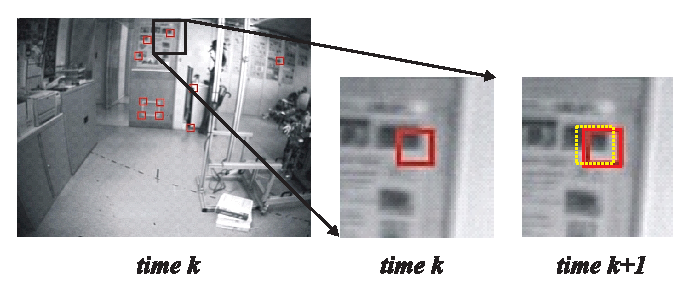
\includegraphics[width=0.75\columnwidth]{images/harris_corners_tracking}
\caption{Example of image features acquisition and tracking using the Harris Corner Detector and Normalized Cross Correlation between two images obtained at consecutive time instants $k$ and $k+1$.}
\label{fig:harris_corners_tracking}
\end{figure}

The features search in the next image was done within a limited region around the previous location of the features to reduce the computation time, assuming the images movement was small enough between two consecutive time instants.

\subsection{Simulated Experiments}\label{sec:simulated_experiments}

It is very difficult to measure the real absolute zero position of each motor joint considering there is no ground-truth for the real robot. One way to evaluate the calibration system in terms of its accuracy is by testing it with simulated experiments. Each experiment simulated the real conditions of the robot and introduced the same level of noise for each sensor according to the values in table \ref{tab:sensors_noise}. It is very important to create simulated environments whose conditions are similar to the real ones.

We performed $5$ experiments where we initialized each joint with different offset values. For each experiment we performed $5$ trials where we simulated the rotation of the robot head. Starting from an arbitrary position, the rotation step for an $i$th joint, $\delta_i^{step}$ was sampled from a Uniform Distribution $\delta_i^{step}\sim\mathcal{U}\left(-\theta,\theta\right)$ with $\theta=0.1$deg. These values were chosen in order to best replicate the real movement that was performed by hand. Between each two steps we sampled $50$ virtual image features by first generating their $3D$ coordinates, within a virtual scenario ranging from $250$mm to $4000$mm, for a certain time instant and calculating their matched coordinates in the consecutive instant by using the complete roto-translation of the head. The virtual image features used as measurements were then obtained by projecting each $3D$ generated point into the corresponding virtual images. Zero-mean Gaussian noise was added to the matched image coordinates, sampled from normal distribution with a standard deviation of $\sigma=2$pixel to simulate the real noise in the matching process.

The results obtained using the proposed algorithm are represented in table \ref{tab:head_offsets_convergence}, with the estimates for experiment $5$ illustrated in figure \ref{fig:head_offsets_convergence} as an example for analysis.

\begin{figure}
\includegraphics[width=0.975\columnwidth]{images/results/calibration_sim_exp_5}
\caption{Simulated experiments: head calibration offsets estimates for experiment $5$ ($5$ trials): Neck tilt $\delta_0$ (in orange), Neck swing $\delta_1$ (in yellow), Neck pan $\delta_2$ (in purple), Eyes tilt $\delta_3$ (in green), Left eye pan $\delta_4$ (in cyan) and Right eye pan $\delta_5$ (in red)}
\label{fig:head_offsets_convergence}
\end{figure}

\begin{table}
\centering
\begin{tabular}{lcccccc}
 \hline
 \# Experiment & $\delta_0$(deg) & $\delta_1$(deg) & $\delta_2$(deg) & $\delta_3$(deg) & $\delta_4$(deg) & $\delta_5$(deg) \\
 \hline
$1$ (ground-truth) & 13.00 & 24.00 & 38.00 & 30.00 & 18.00 & -9.00\\
$1$ (mean) & 13.02 & 23.97 & 38.01 & 31.40 & 17.99 & -7.27\\
$1$ (std) & 0.01 & 0.01 & 0.02 & 0.29 & 0.19 & 0.16 \\
$1$ (mean error) & 0.02 & 0.02 & 0.01 & 1.40 & 0.01 & 1.72\\
 \hline
$2$ (ground-truth) & -9.00 & -11.00 & -35.00 & -39.00 & -24.00 & -9.00\\
$2$ (mean) & -9.01 & -11.02 & -34.98 & -39.11 & -22.49 & -8.36\\
$2$ (std) & 0.01 & 0.02 & 0.03 & 0.41 & 0.17 & 0.40 \\
$2$ (mean error) & 0.01 & 0.02 & 0.01 & 0.12 & 1.50 & 0.63\\
 \hline
$3$ (ground-truth) & -41.00 & -3.00 & 30.00 & -8.00 & -35.00 & 0.00\\
$3$ (mean) & -40.95 & -3.01 & 30.00 & -8.26 & -32.80 & 0.40\\
$3$ (std) & 0.01 & 0.01 & 0.02 & 0.30 & 0.25 & 0.38 \\
$3$ (mean error) & 0.04 & 0.01 & 0.01 & 0.26 & 2.19 & 0.40\\
 \hline
$4$ (ground-truth) & -20.00 & -6.00 & 19.00 & 18.00 & 29.00 & 4.00\\
$4$ (mean) & -19.97 & -6.01 & 19.00 & 19.46 & 28.34 & 4.94\\
$4$ (std) & 0.01 & 0.01 & 0.02 & 0.21 & 0.18 & 0.20 \\
$4$ (mean error) & 0.02 & 0.01 & 1.01 & 1.46 & 0.65 & 0.94\\
 \hline
$5$ (ground-truth) & -14.00 & -5.00 & -56.00 & -43.00 & -33.00 & 12.00\\
$5$ (mean) & -13.99 & -5.01 & -56.01 & -43.14 & -31.55 & 11.67\\
$5$ (std) & 0.02 & 0.01 & 0.02 & 0.38 & 0.27 & 0.46\\
$5$ (mean error) & 0.00 & 0.01 & 0.00 & 0.14 & 1.44 & 0.32\\
 \hline\\
\end{tabular}
\caption{Simulated Experiments: ground-truth and statistical results of the head calibration offsets estimates for $5$ experiments, with $5$ trials each.}
\label{tab:head_offsets_convergence}
\end{table}

\subsubsection{Accuracy}

To evaluate the system in terms of its accuracy we compared the estimates with the ground-truth values represented in table \ref{tab:head_offsets_convergence}. As we can see the error between the real and estimated offsets is very low regardless of the starting position of the head. In this case we have a maximum error of $7\%$ (or $2.19$deg) for the left eye pan joint in experiment $3$. The eyes offsets are the ones presenting the largest errors which can be explained by the approximation taken for the calibration system, where we are assuming the world is static and all points are represented at infinity which may introduce parallax errors that are compensated by the system as errors in the joint space. However we can consider this approximation is still valid for small rotations in short steps between two consecutive time instants, considering our system presents an average error of $0.99$deg for the mentioned eyes joints ($\delta_4$ and $\delta_5$). All the other joints are able to converge to its correct values with much lower errors thus proving the accuracy of the proposed calibration system. 

By observing figure \ref{fig:head_offsets_convergence}, we can see that the system converges in less than $150$ iterations, which considering the lowest sensor runs at $30$Hz and the system works in real time, corresponds to a convergence in less than $5$s. This is very important since the robot can be rapidly calibrated before operation without consuming much of the operator's time. We can see each estimate remains almost constant after convergence, even if the head is continuously rotating. The low standard deviation values represented in table \ref{tab:head_offsets_convergence} show the stability of the system, keeping the estimates as constant as possible under different operation conditions, while the head was being rotated. This is extremely important considering the robot is being calibrated in an online fashion and should keep a well calibrated internal model at all times. 

\subsection{Real Experiments}\label{sec:real_experiments}

The validation of the proposed architecture was very important before testing it in the real robot. The quality of the previous results gave us confidence to test the calibration system in the real robot. Unfortunately, in the real case, there is no ground-truth for the real offsets of the robot. 

We started by performing four experiments (experiments $1$ to $4$) where we initialized the robot head at different arbitrary positions, with a full reset of the encoders between each experiment. For each experiment we performed five trials where we randomly rotated the robot head and eyes by hand during $33.33$ seconds ($1000$ iterations) so as to span most of the range of the robots joints. The mean and standard deviations for each experiment are represented in table \ref{tab:real_head_offsets_convergence}, with the estimates illustrated in figure \ref{fig:head_offsets_convergence_real} for experiment $4$ as an example for analysis.

\begin{figure}
\includegraphics[width=0.975\columnwidth]{images/results/calibration_exp_4}
\caption{Real experiments: head calibration offsets estimates for experiment $4$ ($5$ trials): Neck tilt $\delta_0$ (in orange), Neck swing $\delta_1$ (in yellow), Neck pan $\delta_2$ (in purple), Eyes tilt $\delta_3$ (in green), Left eye pan $\delta_4$ (in cyan) and Right eye pan $\delta_5$ (in red)}
\label{fig:head_offsets_convergence_real}
\end{figure}

\begin{table}
\centering
\begin{tabular}{ccccccc}
 \hline
 $\#$ Exp. & $\delta_0$(deg) & $\delta_1$(deg) & $\delta_2$(deg) & $\delta_3$(deg) & $\delta_4$(deg) & $\delta_5$(deg) \\
 \hline
$1$ (mean) & -41.44 & -41.13 & 62.52 & 3.49 & -48.41 & 44.63 \\
$1$ (std) & 0.60 & 0.68 & 0.73 & 0.11 & 0.35 & 0.27 \\
\hline
$2$ (mean) & -46.82 & 42.91 & 62.82 & 1.34 & -49.22 & -47.00 \\
$2$ (std) & 0.68 & 0.73 & 0.84 & 0.38 & 0.38 & 0.42 \\
\hline
$3$ (mean) & 42.87 & 11.41 & -53.97 & -36.17 & -49.68 & -46.13 \\
$3$ (std) & 0.70 & 0.68 & 0.77 & 0.25 & 0.19 & 0.21 \\
\hline
$4$ (mean) & 41.93 & 35.24 & 61.68 & 34.73 & 46.75 & -46.19 \\
$4$ (std) & 0.64 & 0.68 & 0.85 & 0.49 & 0.34 & 0.36 \\
 \hline\\
\end{tabular}
\caption{Real Experiments: mean and standard deviation values of the offsets estimates for all the experiments ($5$ trials for each experiment)}
\label{tab:real_head_offsets_convergence}
\end{table}

From the figure we can see that the system converged in less than $200$ iterations to very similar estimates under different operation conditions. These results show the capability of the system to correctly calibrate the offsets of the encoders regardless of their starting position, which is of utmost importance for any robotic platform. The low standard deviations for each experiments (maximum value of $0.85$deg), observed in table \ref{tab:real_head_offsets_convergence} also show the stability of the system, which keeps its estimates as constant as possible while the head was being rotated.  

The accuracy of the head calibration system is hard to measure in the real robot, given the lack of ground-truth for each joint. Using the available sensors we measured the accuracy of the neck joints by comparing the real IMU's linear acceleration with the one predicted by the calibrated kinematic model of the robot head. We performed four experiments (experiment $5$ to $8$), with one trial per each, where we initialized the head at different arbitrary positions with a full reset of the encoders between each experiment. After calibration was achieved, for each case the robotic head was homed to the calibrated zero position, using the calibrated offsets to define the absolute zero position of the head. The calibrated offsets and the corresponding recorded gravity vector readings are shown in tables \ref{tab:zero_position_offsets} and \ref{tab:zero_position}, respectively.

\begin{table}
\centering
\begin{tabular}{ccccccc}
 \hline
 $\#$ Exp. & $\delta_0$(deg) & $\delta_1$(deg) & $\delta_2$(deg) & $\delta_3$(deg) & $\delta_4$(deg) & $\delta_5$(deg) \\
 \hline
$5$ & -47.20 & 23.93 & -56.22 & -17.53 & -36.12 & 32.90 \\
$6$ & -34.14 & -35.17 & 49.23 & -19.21 & 38.83 & -40.09 \\
$7$ & 43.80 & -25.82 & 50.91 & -22.91 & 26.51 & -41.99 \\
$8$ & 43.39 & 28.47 & -44.03 & -21.15 & 23.43 & -39.52 \\
 \hline\\
\end{tabular}
\caption{Real Experiments: offsets estimates used to home the head to its zero position}
\label{tab:zero_position_offsets}
\end{table}

\begin{table}
\centering
\begin{tabular}{cccc}
 \hline
 $\#$ Experiment & $g_x$($m/s^2$) & $g_y$($m/s^2$) & $g_z$($m/s^2$) \\
 \hline
$5$ & -0.022 & -9.835 & -0.016 \\
$6$ & 0.034 & -9.844 & -0.096\\
$7$ & -0.102 & -9.829 & -0.091 \\
$8$ & -0.051 & -9.851 & -0.010 \\
 \hline\\
\end{tabular}
\caption{Real Experiments: gravity vector components in the zero position}
\label{tab:zero_position}
\end{table}

We can see that the gravity vector is practically vertical (with an accuracy of 99.99\%) for all four experiments. These results demonstrate the ability of the system to converge to a solution which agrees with the absolute gravity readings, when started in completely different head configurations, thus correctly setting the absolute zero position of the head. After homing to the zero position, for each experiment, we applied a rectangular signal to the neck tilt joint (joint $\delta_0$) in order to compare the real and predicted observations for the gravity vector. The comparison is represented in figure \ref{fig:real_predicted_imu} for experiment $5$ as an example for analysis.

\begin{figure}
 \includegraphics[width=0.975\columnwidth]{images/results/gravity_all}
\caption{Real (red dashed) and predicted (blue solid) gravity vectors for Experiment $5$, with homing to zero position after convergence and response to rectangular signal applied to the first joint, neck tilt.}
\label{fig:real_predicted_imu}
\end{figure}

Figure \ref{fig:real_predicted_imu} correctly shows a leaning forward and backwards pattern, after iteration $1700$, corresponding to the signal applied to the first joint. After convergence of the filter, the predicted and real observations for the gravity vector are correctly aligned, with the prediction matching the real signal in more than $99.9\%$ ot the time. It is important to refer that the IMU is assumed to be perfectly mounted on the top of the head, without any mounting error which may not be true. In that case, the mounting error of the sensor will be reflected in the offsets estimates in order to approximate the real and predicted IMU signals.

\subsubsection{Repeatability}

To better analyse the repeatability of the system, we performed experiment $9$ where we ran the algorithm with the robot head started in six different configurations without a full reset of the encoders, meaning the offsets were the same
for all trials. Figure \ref{fig:offsets_repeatability} shows the convergence of the offset estimates in each trial, with the mean value taken in the last $500$ iterations shown in table \ref{tab:offsets_repeatability} along with the standard deviation of the estimates for all trials. The results show the estimates converging to similar values for different trials, thus empirically proving the robustness of the proposed method to very different starting conditions. The system's repeatability is extremely important to guarantee the quality of the filter, allowing the correct operation of the platform.

\begin{figure}
 \includegraphics[width=0.975\columnwidth]{images/results/repeatability_all}
\caption{Repeatability: head calibration offsets estimates for experiment $9$, with $6$ trials, without a full reset of the encoders, showing the repeatability of the system}
\label{fig:offsets_repeatability}
\end{figure}

\begin{table}
\centering
\begin{tabular}{ccccccc}
 \hline
 $\#$ Trial & $\delta_0$(deg) & $\delta_1$(deg) & $\delta_2$(deg) & $\delta_3$(deg) & $\delta_4$(deg) & $\delta_5$(deg) \\
 \hline
$1$ & -43.8 & 31.7 & -50.2 & -2.1 & 37.3 & -42.4 \\
$2$ & -43.4 & 32.6 & -52.7 & -3.4 & 35.5 & -43.7 \\
$3$ & -43.4 & 31.4 & -50.9 & -1.5 & 36.9 & -40.4 \\
$4$ & -43.1 & 32.0 & -52.0 & -3.9 & 37.4 & -42.2 \\
$5$ & -43.4 & 32.8 & -51.1 & -2.3 & 39.8 & -42.1 \\
$6$ & -43.0 & 33.0 & -52.9 & -3.9 & 35.7 & -41.6 \\
 \hline
mean & -43.57 &  32.31 & -50.54 & -2.72 & 36.85 & -42.20 \\
std & 0.28 & 0.64 & 1.07 & 1.02 & 1.54 & 1.08 \\
 \hline \\
\end{tabular}
\caption{Repatability: mean values of the offsets estimates for experiment $9$, with $6$ trials, without a full reset of the encoders}
\label{tab:offsets_repeatability}
\end{table}

It is worth noting, in figure \ref{fig:offsets_repeatability}, that immediately after the first iteration the system has already assimilated the first reading of the accelerometer. Since different head configurations can provide the same accelerometer readings (e.g. different pan angles with a fully upright head), the initial measurements are not enough to converge to the final configuration nor do they provide any information about the eye joints. The head movements are required to disambiguate these multiple solutions and provide the final offsets values, as seen by the rapid convergence of the filter after rotating the head.

During operation we noticed there were backlash zones in some of the joints, specially those carrying most of the weight. Within these backlash zones the encoders can not provide any measurements even though the joint is rotating in its motor shaft. However, the backlash was not reflected in the final estimates which shows that our system can adapt to sudden changes and perturbation that may occur during operation, mainly due to sensor fusion. The IMU and the cameras could perceive movement even though the encoders were telling the exact opposite. Sensor fusion is extremely useful to increase the robustness of the system in several situations where one or more sensors could fail. This case is a clear example of how multiple sensors integrated into a single architecture generate a better response than each one of them separated.